\chapter{Introduction to Complex Systems}
Complex systems are interdisciplinary: you have to communicate your results to experts from different science field.
You need to provide an easy answer to a complex problem, no matter how difficult it's to get this answer.

\section{Emergence}
One of the main ideas in complex systems is emergence. Emergence means that the structure of the particles is simple and they are not so important like interactions bettween them. \\
An example of this is the Central limit therem, which comes from mathematics. \\ \\
If you have a random variable $x_k$, with average value $\lang x_k \rang = 0$ and finite variance $\sigma^2$, then the central limit theorem says that, if the variables are independent (and in physics this is usally a fair assumption) for every value of $k$, then the normalized sum 
$$
	z_n = \frac{1}{\sqrt{N}}\sum_{k=0}^N x_k
$$
then the distribution of this variable $z_n$ is known, and it is gaussian, for a big enough value of $N$.
$$
	\rho(z_n) \sim \exp\left(-\frac{z^2}{2\sigma^2}\right)
$$
Despite the fact that we, as humans, need a cause-effect relationship to describe a phenomenon, nature loves independent events, like DNA mutations.
The gaussian describes the fluctuations of a system at equilibrium, not the complexity. You cannot extract work from fluctuations at equilibrium, otherwise you violate thermodynamics (and that's no good). \\
The gaussian function is not a physical function, because it implies non zero probabilities to events which are impossible. For example, if we take a particle in a basin of attraction of a potential, the non zero probability given by the gaussian fluctuations allows the particle to jump out of the pit. But this violates the second law of thermodynamics. \\ \\
A way to defy the gaussian properties is to allow a system to have memory, so to remove the independence of the variable. 
\begin{center}
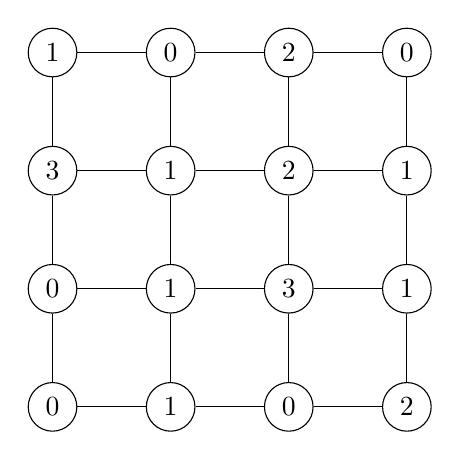
\begin{tikzpicture}[node distance={15mm}, main/.style = {draw,circle}]
\node[main] (1) {1};
\node[main] (2) [right of=1] {0};
\node[main] (3) [right of=2] {2};
\node[main] (4) [right of =3] {0};
\node[main] (5) [below of =1] {3};
\node[main] (6) [right of=5] {1};
\node[main] (7) [right of=6] {2};
\node[main] (8) [right of=7] {1};
\node[main] (9) [below of=5] {0};
\node[main] (10) [right of=9] {1};
\node[main] (11) [right of=10] {3};
\node[main] (12) [right of=11] {1};
\node[main] (13) [below of=9] {0};
\node[main] (14) [right of=13] {1};
\node[main] (15) [right of=14] {0};
\node[main] (16) [right of=15] {2};
\draw (1) -- (2);
\draw (1) -- (5);
\draw (2) -- (3);
\draw (3) -- (4);
\draw (5) -- (6);
\draw (6) -- (7);
\draw (7) -- (8);
\draw (5) -- (9);
\draw (9) -- (10);
\draw (10) -- (11);
\draw (11) -- (12);
\draw (9) -- (13);
\draw (13) -- (14);
\draw (14) -- (15);
\draw (15) -- (16);
\draw (2) -- (6);
\draw (3) -- (7);
\draw (4) -- (8);
\draw (6) -- (10);
\draw (7) -- (11);
\draw (8) -- (12);
\draw (10) -- (14);
\draw (11) -- (15);
\draw (12) -- (16);
\end{tikzpicture}
\end{center}
One example of this is the sand pile model. You have a lattice, and each point is connected to its four neighbors. At this point one particle is put in a randomly chosen point. Each node can have four possible states, $0,1,2,3$, that is four possible numbers of particles. If a node reaches 4 particles, the 4 particles are distributed to the 4 neightbouring nodes.
\begin{center}
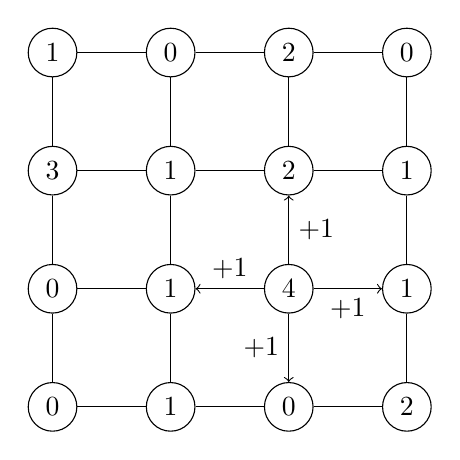
\begin{tikzpicture}[node distance={15mm}, main/.style = {draw,circle}]
\node[main] (1) {1};
\node[main] (2) [right of=1] {0};
\node[main] (3) [right of=2] {2};
\node[main] (4) [right of =3] {0};
\node[main] (5) [below of =1] {3};
\node[main] (6) [right of=5] {1};
\node[main] (7) [right of=6] {2};
\node[main] (8) [right of=7] {1};
\node[main] (9) [below of=5] {0};
\node[main] (10) [right of=9] {1};
\node[main] (11) [right of=10] {4};
\node[main] (12) [right of=11] {1};
\node[main] (13) [below of=9] {0};
\node[main] (14) [right of=13] {1};
\node[main] (15) [right of=14] {0};
\node[main] (16) [right of=15] {2};
\draw (1) -- (2);
\draw (1) -- (5);
\draw (2) -- (3);
\draw (3) -- (4);
\draw (5) -- (6);
\draw (6) -- (7);
\draw (7) -- (8);
\draw (5) -- (9);
\draw (9) -- (10);
\draw[->] (11) -- node[above]{+1} (10);
\draw[->] (11) -- node[below]{+1} (12);
\draw (9) -- (13);
\draw (13) -- (14);
\draw (14) -- (15);
\draw (15) -- (16);
\draw (2) -- (6);
\draw (3) -- (7);
\draw (4) -- (8);
\draw (6) -- (10);
\draw[->] (11) -- node[right]{+1} (7);
\draw (8) -- (12);
\draw (10) -- (14);
\draw[->] (11) -- node[left]{+1} (15);
\draw (12) -- (16);
\end{tikzpicture}
\end{center}
\begin{center}
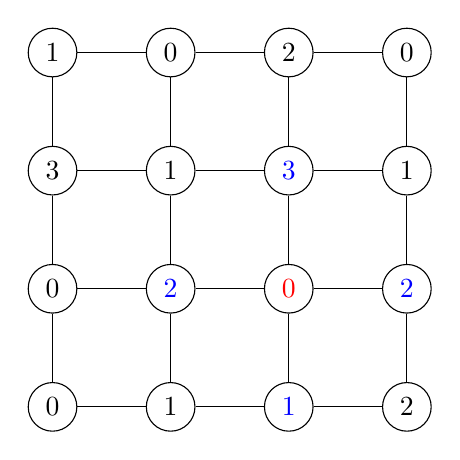
\begin{tikzpicture}[node distance={15mm}, main/.style = {draw,circle}]
\node[main] (1) {1};
\node[main] (2) [right of=1] {0};
\node[main] (3) [right of=2] {2};
\node[main] (4) [right of =3] {0};
\node[main] (5) [below of =1] {3};
\node[main] (6) [right of=5] {1};
\node[main] (7) [right of=6] {\textcolor{blue}{3}};
\node[main] (8) [right of=7] {1};
\node[main] (9) [below of=5] {0};
\node[main] (10) [right of=9] {\textcolor{blue}{2}};
\node[main] (11) [right of=10] {\textcolor{red}{0}};
\node[main] (12) [right of=11] {\textcolor{blue}{2}};
\node[main] (13) [below of=9] {0};
\node[main] (14) [right of=13] {1};
\node[main] (15) [right of=14] {\textcolor{blue}{1}};
\node[main] (16) [right of=15] {2};
\draw (1) -- (2);
\draw (1) -- (5);
\draw (2) -- (3);
\draw (3) -- (4);
\draw (5) -- (6);
\draw (6) -- (7);
\draw (7) -- (8);
\draw (5) -- (9);
\draw (9) -- (10);
\draw (11) -- (10);
\draw (11) -- (12);
\draw (9) -- (13);
\draw (13) -- (14);
\draw (14) -- (15);
\draw (15) -- (16);
\draw (2) -- (6);
\draw (3) -- (7);
\draw (4) -- (8);
\draw (6) -- (10);
\draw (11) -- (7);
\draw (8) -- (12);
\draw (10) -- (14);
\draw (11) --  (15);
\draw (12) -- (16);
\end{tikzpicture}
\end{center}
For the nodes in the border, what happens is that 2 of the particles are redistributed and the other 2 are released in the enviroment, so they are lost. \\ \\
So this system has memory, and this means that the states of all the nodes are not independent. This memory turns the gaussian distribution into a power law
$$
	p(n) \propto n^{-\alpha}
$$
with $\alpha > 1$. \\
The decay of the power low is much much slower than that of the gaussian, which means that the probability to have events in the extremes is significantly higher with the power low distribution.
Memory is related to power laws, but viceversa is not guaranteed.
We can also have power laws in physics, for example in the Ising model.
In physics, power laws tipically represent a phase transition for a dynamic system in a non-equilibrium state. \\
In the sand pile model, we notice a self-organized criticality: the system naturally goes into a critical state and does a phase transition. \\
Another example of a natural power law is the Kleiber law wich relates the metabolic rate (amount of energy you need to survive) to the mass.
\begin{equation}
	E(m) \propto m^{\frac{4}{3}}
\end{equation}
We can also observe that heartbeat rate decreases with mass and lifetime increases.
\section{The broken stick model}
Let's consider the portion $[0,1]$ of the axis, which represents a segment (a stick) of length 1. Suppose that we extract randomically a point $x_1$ on that segment, and we cut it in correspondence of that point, thus obtaining the portion $[0,x_1]$ of the axis. \\
By repeating this process many times, we obtain a system with memory, because of course the length of the segment at a certain iteration depends on all the previous iterations. \\
This is called the broken stick model. \\
For this system one expects to have a power law distribution, because if we rescale the variable $x$, the distribution must not change.
$$
	p(x) \sim \frac{1}{x^a}
$$
$$
	y = \la x \ \ \longrightarrow \ \ p(y) = \frac{1}{(\la x)^a} \sim \frac{1}{x^a}
$$
Since we have:
$$
	\lang x_k \rang = \frac{\lang x_{k-1} \rang}{2}
$$
$$
	\rho_N(2x) = \frac{1}{2}\rho_{N-1}(x)
$$
Which means that, as $N$ goes to infinity we get
$$
	\rho(2x) = \frac{1}{2}\rho(x)
$$
$$
	\rho(x) = \frac{1}{x}
$$
Let's now try to implement the system without memory. So we have $N$ independent variables $x_k$ uniformly distributed, and for each variable we define its distance from the previous one, $\Delta x$. \\
The probability to find $\Delta x$ is the probability of not finding $x$ in any segment, so
$$
	p(\Delta x) \approx \left( 1 - \frac{\Delta x}{L} \right)
$$
We then take a new variable $y = N\Delta x$ and we obtain the probability distribution
$$
	p = \exp(-y/L)
$$
as $N$ goes to infinity, which of course is an exponential law. \\ \\
Suppose that the whole stick is a state, and we want to distribute the population inside of it. If we divide the stick uniformly in portions and diivde the populations in this group, we obtain an exponential law, as we have just seen. \\
Another way, which contains memory, consists of creating a city and letting it grow, and only then introducing a second one, and repeating the process until all the space is occupied. 
\chapter{Total energy in a network}
Let's take a region of space containing a number $N$ of nodes. This system can represent, for example, the hydraulic network of a city. 
For a node we define its "energy" flow $\varphi$ (in the case of the hydraulic network, what is flowing between the nodes is water). How much "energy" do we need to insert in the system? \\
If we have to distribute something to all the nodes, the most basic way to do it is to connect one on one all the nodes, as to form a long chain. \\
\begin{center}
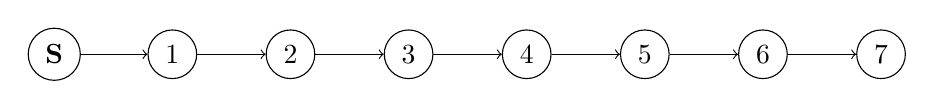
\begin{tikzpicture}[node distance={15mm}, main/.style = {draw,circle}]
\node[main] (1) {1};
\node[main] (0) [left of=1] {\textbf{S}};
\node[main] (2) [right of=1] {2};
\node[main] (3) [right of=2] {3};
\node[main] (4) [right of =3] {4};
\node[main] (5) [right of =4] {5};
\node[main] (6) [right of=5] {6};
\node[main] (7) [right of=6] {7};
\draw[->] (0) -- (1);
\draw[->] (1) -- (2);
\draw[->] (2) -- (3);
\draw[->] (3) -- (4);
\draw[->] (4) -- (5);
\draw[->] (5) -- (6);
\draw[->] (6) -- (7);
\end{tikzpicture}
\end{center}
If the flow out of the source $S$ is $\phi$, the flow after the first node is $\phi - \varphi$, and so on, and we expect that the flow arriving to the final node will be $\varphi$. \\
So the total energy is 
$$
	E_T \approx l\sum_{k=0}^{N-1} (\phi - k\varphi) = l\varphi\sum_{k=0}^{N-1} k`
$$
$$
	E_T \propto l\varphi N^2
$$
So the totaly energy that is required to provide for all the nodes, with this configuration, is proportional to the square of the total number of nodes. So with this configuration we have a network that is very easy to implement, but the network is very inefficient. \\ \\ 
Another possible connection of the nodes is the following one:
\begin{center}
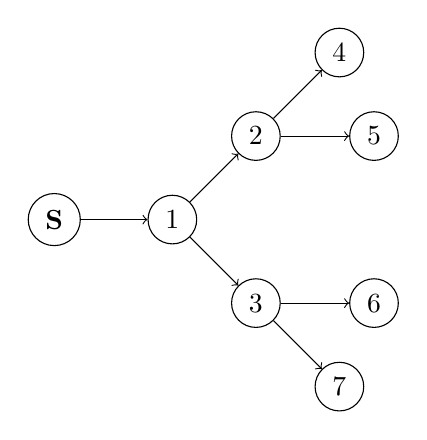
\begin{tikzpicture}[node distance={15mm}, main/.style = {draw,circle}]
\node[main] (1) {1};
\node[main] (0) [left of=1] {\textbf{S}};
\node[main] (2) [above right of=1] {2};
\node[main] (3) [below right of=1] {3};
\node[main] (4) [above right of =2] {4};
\node[main] (5) [right of =2] {5};
\node[main] (6) [right of=3] {6};
\node[main] (7) [below right of=3] {7};
\draw[->] (0) -- (1);
\draw[->] (1) -- (2);
\draw[->]  (1) -- (3);
\draw[->]  (2) -- (4);
\draw[->]  (2) -- (5);
\draw[->]  (3) -- (6);
\draw[->]  (3) -- (7);
\end{tikzpicture}
\end{center}
So each node is linked to two mode nodes. This is what is called a tree structure. \\
The main problem with such a structure is that the path between the nodes is always the same, but it is impossible to design a city in such a way. \\
The number of nodes is $2^m$, where $m$ is the number of levels, so one has that $2^{m+1} = N$. \\
The relation for the flow in each level is
$$
	2\phi_k + \varphi = \phi_{k-1}
$$
where we assume again that the flow in the final level is $\varphi$. \\
$\phi_k$ then is
$$
	\phi_k = (2^{m+1-k}-1)\varphi
$$
Then:
$$
	E_T = d\varphi\sum_{k=1}^m 2^k(2^{m+1-k}-1) \approx d\varphi m 2^{m+1}	
$$
$$
	E_T = d\phi N \log_2(N)
$$
This configuration is much more efficient than the previous alternative, although it is impossible to put to practice. \\ \\ 
So we need to find a solution that is in the middle of these two. 
